% Options for packages loaded elsewhere
\PassOptionsToPackage{unicode}{hyperref}
\PassOptionsToPackage{hyphens}{url}
\PassOptionsToPackage{dvipsnames,svgnames,x11names}{xcolor}
%
\documentclass[
  letterpaper,
  DIV=11,
  numbers=noendperiod]{scrartcl}

\usepackage{amsmath,amssymb}
\usepackage{iftex}
\ifPDFTeX
  \usepackage[T1]{fontenc}
  \usepackage[utf8]{inputenc}
  \usepackage{textcomp} % provide euro and other symbols
\else % if luatex or xetex
  \usepackage{unicode-math}
  \defaultfontfeatures{Scale=MatchLowercase}
  \defaultfontfeatures[\rmfamily]{Ligatures=TeX,Scale=1}
\fi
\usepackage{lmodern}
\ifPDFTeX\else  
    % xetex/luatex font selection
\fi
% Use upquote if available, for straight quotes in verbatim environments
\IfFileExists{upquote.sty}{\usepackage{upquote}}{}
\IfFileExists{microtype.sty}{% use microtype if available
  \usepackage[]{microtype}
  \UseMicrotypeSet[protrusion]{basicmath} % disable protrusion for tt fonts
}{}
\makeatletter
\@ifundefined{KOMAClassName}{% if non-KOMA class
  \IfFileExists{parskip.sty}{%
    \usepackage{parskip}
  }{% else
    \setlength{\parindent}{0pt}
    \setlength{\parskip}{6pt plus 2pt minus 1pt}}
}{% if KOMA class
  \KOMAoptions{parskip=half}}
\makeatother
\usepackage{xcolor}
\setlength{\emergencystretch}{3em} % prevent overfull lines
\setcounter{secnumdepth}{-\maxdimen} % remove section numbering
% Make \paragraph and \subparagraph free-standing
\ifx\paragraph\undefined\else
  \let\oldparagraph\paragraph
  \renewcommand{\paragraph}[1]{\oldparagraph{#1}\mbox{}}
\fi
\ifx\subparagraph\undefined\else
  \let\oldsubparagraph\subparagraph
  \renewcommand{\subparagraph}[1]{\oldsubparagraph{#1}\mbox{}}
\fi

\usepackage{color}
\usepackage{fancyvrb}
\newcommand{\VerbBar}{|}
\newcommand{\VERB}{\Verb[commandchars=\\\{\}]}
\DefineVerbatimEnvironment{Highlighting}{Verbatim}{commandchars=\\\{\}}
% Add ',fontsize=\small' for more characters per line
\usepackage{framed}
\definecolor{shadecolor}{RGB}{241,243,245}
\newenvironment{Shaded}{\begin{snugshade}}{\end{snugshade}}
\newcommand{\AlertTok}[1]{\textcolor[rgb]{0.68,0.00,0.00}{#1}}
\newcommand{\AnnotationTok}[1]{\textcolor[rgb]{0.37,0.37,0.37}{#1}}
\newcommand{\AttributeTok}[1]{\textcolor[rgb]{0.40,0.45,0.13}{#1}}
\newcommand{\BaseNTok}[1]{\textcolor[rgb]{0.68,0.00,0.00}{#1}}
\newcommand{\BuiltInTok}[1]{\textcolor[rgb]{0.00,0.23,0.31}{#1}}
\newcommand{\CharTok}[1]{\textcolor[rgb]{0.13,0.47,0.30}{#1}}
\newcommand{\CommentTok}[1]{\textcolor[rgb]{0.37,0.37,0.37}{#1}}
\newcommand{\CommentVarTok}[1]{\textcolor[rgb]{0.37,0.37,0.37}{\textit{#1}}}
\newcommand{\ConstantTok}[1]{\textcolor[rgb]{0.56,0.35,0.01}{#1}}
\newcommand{\ControlFlowTok}[1]{\textcolor[rgb]{0.00,0.23,0.31}{#1}}
\newcommand{\DataTypeTok}[1]{\textcolor[rgb]{0.68,0.00,0.00}{#1}}
\newcommand{\DecValTok}[1]{\textcolor[rgb]{0.68,0.00,0.00}{#1}}
\newcommand{\DocumentationTok}[1]{\textcolor[rgb]{0.37,0.37,0.37}{\textit{#1}}}
\newcommand{\ErrorTok}[1]{\textcolor[rgb]{0.68,0.00,0.00}{#1}}
\newcommand{\ExtensionTok}[1]{\textcolor[rgb]{0.00,0.23,0.31}{#1}}
\newcommand{\FloatTok}[1]{\textcolor[rgb]{0.68,0.00,0.00}{#1}}
\newcommand{\FunctionTok}[1]{\textcolor[rgb]{0.28,0.35,0.67}{#1}}
\newcommand{\ImportTok}[1]{\textcolor[rgb]{0.00,0.46,0.62}{#1}}
\newcommand{\InformationTok}[1]{\textcolor[rgb]{0.37,0.37,0.37}{#1}}
\newcommand{\KeywordTok}[1]{\textcolor[rgb]{0.00,0.23,0.31}{#1}}
\newcommand{\NormalTok}[1]{\textcolor[rgb]{0.00,0.23,0.31}{#1}}
\newcommand{\OperatorTok}[1]{\textcolor[rgb]{0.37,0.37,0.37}{#1}}
\newcommand{\OtherTok}[1]{\textcolor[rgb]{0.00,0.23,0.31}{#1}}
\newcommand{\PreprocessorTok}[1]{\textcolor[rgb]{0.68,0.00,0.00}{#1}}
\newcommand{\RegionMarkerTok}[1]{\textcolor[rgb]{0.00,0.23,0.31}{#1}}
\newcommand{\SpecialCharTok}[1]{\textcolor[rgb]{0.37,0.37,0.37}{#1}}
\newcommand{\SpecialStringTok}[1]{\textcolor[rgb]{0.13,0.47,0.30}{#1}}
\newcommand{\StringTok}[1]{\textcolor[rgb]{0.13,0.47,0.30}{#1}}
\newcommand{\VariableTok}[1]{\textcolor[rgb]{0.07,0.07,0.07}{#1}}
\newcommand{\VerbatimStringTok}[1]{\textcolor[rgb]{0.13,0.47,0.30}{#1}}
\newcommand{\WarningTok}[1]{\textcolor[rgb]{0.37,0.37,0.37}{\textit{#1}}}

\providecommand{\tightlist}{%
  \setlength{\itemsep}{0pt}\setlength{\parskip}{0pt}}\usepackage{longtable,booktabs,array}
\usepackage{calc} % for calculating minipage widths
% Correct order of tables after \paragraph or \subparagraph
\usepackage{etoolbox}
\makeatletter
\patchcmd\longtable{\par}{\if@noskipsec\mbox{}\fi\par}{}{}
\makeatother
% Allow footnotes in longtable head/foot
\IfFileExists{footnotehyper.sty}{\usepackage{footnotehyper}}{\usepackage{footnote}}
\makesavenoteenv{longtable}
\usepackage{graphicx}
\makeatletter
\def\maxwidth{\ifdim\Gin@nat@width>\linewidth\linewidth\else\Gin@nat@width\fi}
\def\maxheight{\ifdim\Gin@nat@height>\textheight\textheight\else\Gin@nat@height\fi}
\makeatother
% Scale images if necessary, so that they will not overflow the page
% margins by default, and it is still possible to overwrite the defaults
% using explicit options in \includegraphics[width, height, ...]{}
\setkeys{Gin}{width=\maxwidth,height=\maxheight,keepaspectratio}
% Set default figure placement to htbp
\makeatletter
\def\fps@figure{htbp}
\makeatother

\KOMAoption{captions}{tableheading}
\makeatletter
\makeatother
\makeatletter
\makeatother
\makeatletter
\@ifpackageloaded{caption}{}{\usepackage{caption}}
\AtBeginDocument{%
\ifdefined\contentsname
  \renewcommand*\contentsname{Table of contents}
\else
  \newcommand\contentsname{Table of contents}
\fi
\ifdefined\listfigurename
  \renewcommand*\listfigurename{List of Figures}
\else
  \newcommand\listfigurename{List of Figures}
\fi
\ifdefined\listtablename
  \renewcommand*\listtablename{List of Tables}
\else
  \newcommand\listtablename{List of Tables}
\fi
\ifdefined\figurename
  \renewcommand*\figurename{Figure}
\else
  \newcommand\figurename{Figure}
\fi
\ifdefined\tablename
  \renewcommand*\tablename{Table}
\else
  \newcommand\tablename{Table}
\fi
}
\@ifpackageloaded{float}{}{\usepackage{float}}
\floatstyle{ruled}
\@ifundefined{c@chapter}{\newfloat{codelisting}{h}{lop}}{\newfloat{codelisting}{h}{lop}[chapter]}
\floatname{codelisting}{Listing}
\newcommand*\listoflistings{\listof{codelisting}{List of Listings}}
\makeatother
\makeatletter
\@ifpackageloaded{caption}{}{\usepackage{caption}}
\@ifpackageloaded{subcaption}{}{\usepackage{subcaption}}
\makeatother
\makeatletter
\@ifpackageloaded{tcolorbox}{}{\usepackage[skins,breakable]{tcolorbox}}
\makeatother
\makeatletter
\@ifundefined{shadecolor}{\definecolor{shadecolor}{rgb}{.97, .97, .97}}
\makeatother
\makeatletter
\makeatother
\makeatletter
\makeatother
\ifLuaTeX
  \usepackage{selnolig}  % disable illegal ligatures
\fi
\IfFileExists{bookmark.sty}{\usepackage{bookmark}}{\usepackage{hyperref}}
\IfFileExists{xurl.sty}{\usepackage{xurl}}{} % add URL line breaks if available
\urlstyle{same} % disable monospaced font for URLs
\hypersetup{
  pdftitle={Class 18: Pertussis Mini-Project},
  pdfauthor={Raquel Gonzalez (A16207442)},
  colorlinks=true,
  linkcolor={blue},
  filecolor={Maroon},
  citecolor={Blue},
  urlcolor={Blue},
  pdfcreator={LaTeX via pandoc}}

\title{Class 18: Pertussis Mini-Project}
\author{Raquel Gonzalez (A16207442)}
\date{}

\begin{document}
\maketitle
\ifdefined\Shaded\renewenvironment{Shaded}{\begin{tcolorbox}[interior hidden, borderline west={3pt}{0pt}{shadecolor}, boxrule=0pt, sharp corners, frame hidden, enhanced, breakable]}{\end{tcolorbox}}\fi

First we will examine and explore Pertussis case numbers in the U.S. as
tracked by the CDC:
https://www.cdc.gov/pertussis/surv-reporting/cases-by-year.html

We can use the datapasta package to scrape this data from the website
into R:

\begin{Shaded}
\begin{Highlighting}[]
\NormalTok{cdc }\OtherTok{\textless{}{-}} \FunctionTok{data.frame}\NormalTok{(}\AttributeTok{year =} \FunctionTok{c}\NormalTok{(1922L,1923L,1924L,1925L,}
\NormalTok{                                          1926L,1927L,1928L,1929L,1930L,1931L,}
\NormalTok{                                          1932L,1933L,1934L,1935L,1936L,}
\NormalTok{                                          1937L,1938L,1939L,1940L,1941L,1942L,}
\NormalTok{                                          1943L,1944L,1945L,1946L,1947L,}
\NormalTok{                                          1948L,1949L,1950L,1951L,1952L,}
\NormalTok{                                          1953L,1954L,1955L,1956L,1957L,1958L,}
\NormalTok{                                          1959L,1960L,1961L,1962L,1963L,}
\NormalTok{                                          1964L,1965L,1966L,1967L,1968L,1969L,}
\NormalTok{                                          1970L,1971L,1972L,1973L,1974L,}
\NormalTok{                                          1975L,1976L,1977L,1978L,1979L,1980L,}
\NormalTok{                                          1981L,1982L,1983L,1984L,1985L,}
\NormalTok{                                          1986L,1987L,1988L,1989L,1990L,}
\NormalTok{                                          1991L,1992L,1993L,1994L,1995L,1996L,}
\NormalTok{                                          1997L,1998L,1999L,2000L,2001L,}
\NormalTok{                                          2002L,2003L,2004L,2005L,2006L,2007L,}
\NormalTok{                                          2008L,2009L,2010L,2011L,2012L,}
\NormalTok{                                          2013L,2014L,2015L,2016L,2017L,2018L,}
                                          
\NormalTok{2019L,2020L,2021L),}

\AttributeTok{cases =} \FunctionTok{c}\NormalTok{(}\DecValTok{107473}\NormalTok{,}\DecValTok{164191}\NormalTok{,}\DecValTok{165418}\NormalTok{,}\DecValTok{152003}\NormalTok{,}
                                          \DecValTok{202210}\NormalTok{,}\DecValTok{181411}\NormalTok{,}\DecValTok{161799}\NormalTok{,}\DecValTok{197371}\NormalTok{,}
                                          \DecValTok{166914}\NormalTok{,}\DecValTok{172559}\NormalTok{,}\DecValTok{215343}\NormalTok{,}\DecValTok{179135}\NormalTok{,}\DecValTok{265269}\NormalTok{,}
                                          \DecValTok{180518}\NormalTok{,}\DecValTok{147237}\NormalTok{,}\DecValTok{214652}\NormalTok{,}\DecValTok{227319}\NormalTok{,}\DecValTok{103188}\NormalTok{,}
                                          \DecValTok{183866}\NormalTok{,}\DecValTok{222202}\NormalTok{,}\DecValTok{191383}\NormalTok{,}\DecValTok{191890}\NormalTok{,}\DecValTok{109873}\NormalTok{,}
                                          \DecValTok{133792}\NormalTok{,}\DecValTok{109860}\NormalTok{,}\DecValTok{156517}\NormalTok{,}\DecValTok{74715}\NormalTok{,}\DecValTok{69479}\NormalTok{,}
                                          \DecValTok{120718}\NormalTok{,}\DecValTok{68687}\NormalTok{,}\DecValTok{45030}\NormalTok{,}\DecValTok{37129}\NormalTok{,}\DecValTok{60886}\NormalTok{,}
                                          \DecValTok{62786}\NormalTok{,}\DecValTok{31732}\NormalTok{,}\DecValTok{28295}\NormalTok{,}\DecValTok{32148}\NormalTok{,}\DecValTok{40005}\NormalTok{,}
                                          \DecValTok{14809}\NormalTok{,}\DecValTok{11468}\NormalTok{,}\DecValTok{17749}\NormalTok{,}\DecValTok{17135}\NormalTok{,}\DecValTok{13005}\NormalTok{,}\DecValTok{6799}\NormalTok{,}
                                          \DecValTok{7717}\NormalTok{,}\DecValTok{9718}\NormalTok{,}\DecValTok{4810}\NormalTok{,}\DecValTok{3285}\NormalTok{,}\DecValTok{4249}\NormalTok{,}\DecValTok{3036}\NormalTok{,}
                                          \DecValTok{3287}\NormalTok{,}\DecValTok{1759}\NormalTok{,}\DecValTok{2402}\NormalTok{,}\DecValTok{1738}\NormalTok{,}\DecValTok{1010}\NormalTok{,}\DecValTok{2177}\NormalTok{,}\DecValTok{2063}\NormalTok{,}
                                          \DecValTok{1623}\NormalTok{,}\DecValTok{1730}\NormalTok{,}\DecValTok{1248}\NormalTok{,}\DecValTok{1895}\NormalTok{,}\DecValTok{2463}\NormalTok{,}\DecValTok{2276}\NormalTok{,}
                                          \DecValTok{3589}\NormalTok{,}\DecValTok{4195}\NormalTok{,}\DecValTok{2823}\NormalTok{,}\DecValTok{3450}\NormalTok{,}\DecValTok{4157}\NormalTok{,}\DecValTok{4570}\NormalTok{,}
                                          \DecValTok{2719}\NormalTok{,}\DecValTok{4083}\NormalTok{,}\DecValTok{6586}\NormalTok{,}\DecValTok{4617}\NormalTok{,}\DecValTok{5137}\NormalTok{,}\DecValTok{7796}\NormalTok{,}\DecValTok{6564}\NormalTok{,}
                                          \DecValTok{7405}\NormalTok{,}\DecValTok{7298}\NormalTok{,}\DecValTok{7867}\NormalTok{,}\DecValTok{7580}\NormalTok{,}\DecValTok{9771}\NormalTok{,}\DecValTok{11647}\NormalTok{,}
                                          \DecValTok{25827}\NormalTok{,}\DecValTok{25616}\NormalTok{,}\DecValTok{15632}\NormalTok{,}\DecValTok{10454}\NormalTok{,}\DecValTok{13278}\NormalTok{,}
                                          \DecValTok{16858}\NormalTok{,}\DecValTok{27550}\NormalTok{,}\DecValTok{18719}\NormalTok{,}\DecValTok{48277}\NormalTok{,}\DecValTok{28639}\NormalTok{,}\DecValTok{32971}\NormalTok{,}
                                          \DecValTok{20762}\NormalTok{,}\DecValTok{17972}\NormalTok{,}\DecValTok{18975}\NormalTok{,}\DecValTok{15609}\NormalTok{,}\DecValTok{18617}\NormalTok{,}

\DecValTok{6124}\NormalTok{,}\DecValTok{2116}\NormalTok{))}
\end{Highlighting}
\end{Shaded}

\begin{Shaded}
\begin{Highlighting}[]
\FunctionTok{head}\NormalTok{(cdc)}
\end{Highlighting}
\end{Shaded}

\begin{verbatim}
  year  cases
1 1922 107473
2 1923 164191
3 1924 165418
4 1925 152003
5 1926 202210
6 1927 181411
\end{verbatim}

\begin{quote}
Q1: With the help of the R ``addin'' package datapasta assign the CDC
pertussis case number data to a data frame called cdc and use ggplot to
make a plot of cases numbers over time.
\end{quote}

I want a plot of cases per year with ggplot.

\begin{Shaded}
\begin{Highlighting}[]
\FunctionTok{library}\NormalTok{(ggplot2)}
\end{Highlighting}
\end{Shaded}

\begin{Shaded}
\begin{Highlighting}[]
\FunctionTok{ggplot}\NormalTok{(cdc) }\SpecialCharTok{+}
  \FunctionTok{aes}\NormalTok{(year, cases) }\SpecialCharTok{+}
  \FunctionTok{geom\_line}\NormalTok{()}
\end{Highlighting}
\end{Shaded}

\begin{figure}[H]

{\centering 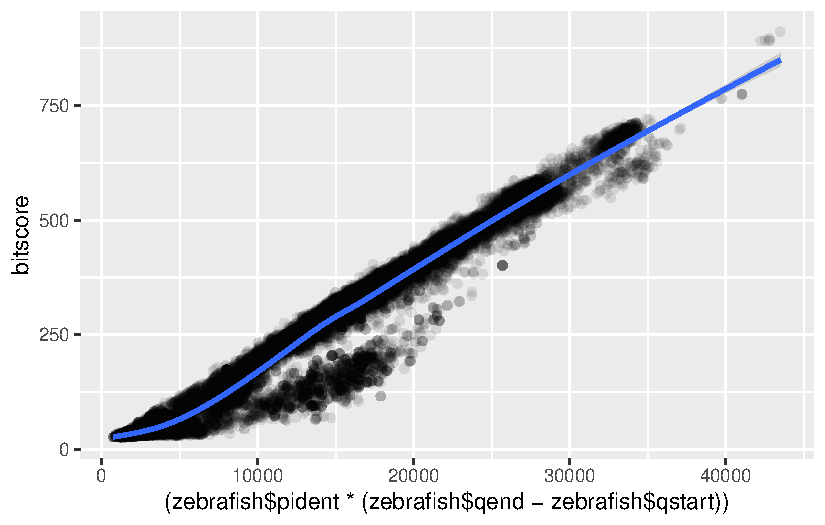
\includegraphics{class18_files/figure-pdf/unnamed-chunk-4-1.pdf}

}

\end{figure}

\begin{quote}
Q2. Using the ggplot geom\_vline() function add lines to your previous
plot for the 1946 introduction of the wP vaccine and the 1996 switch to
aP vaccine (see example in the hint below). What do you notice?
\end{quote}

\begin{Shaded}
\begin{Highlighting}[]
\FunctionTok{ggplot}\NormalTok{(cdc) }\SpecialCharTok{+}
  \FunctionTok{aes}\NormalTok{(year, cases) }\SpecialCharTok{+}
  \FunctionTok{geom\_line}\NormalTok{() }\SpecialCharTok{+}
  \FunctionTok{geom\_vline}\NormalTok{(}\AttributeTok{xintercept=}\DecValTok{1947}\NormalTok{, }\AttributeTok{col=}\StringTok{"blue"}\NormalTok{) }\SpecialCharTok{+}
  \FunctionTok{geom\_vline}\NormalTok{(}\AttributeTok{xintercept=}\DecValTok{1992}\NormalTok{, }\AttributeTok{col=}\StringTok{"purple"}\NormalTok{) }\SpecialCharTok{+}
  \FunctionTok{geom\_vline}\NormalTok{(}\AttributeTok{xintercept=}\DecValTok{2020}\NormalTok{, }\AttributeTok{col=}\StringTok{"magenta"}\NormalTok{)}
\end{Highlighting}
\end{Shaded}

\begin{figure}[H]

{\centering 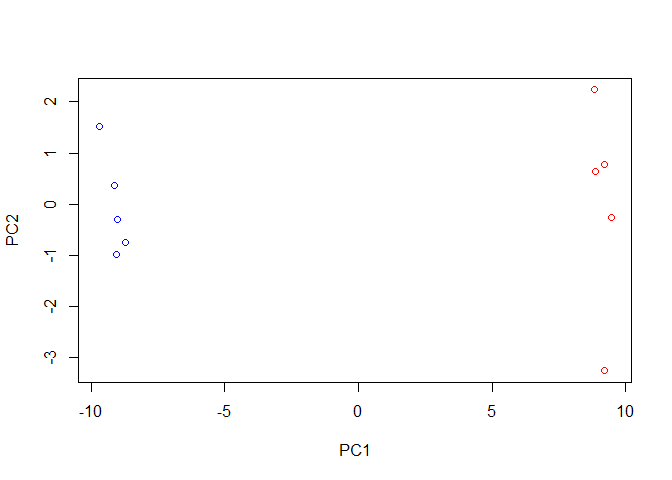
\includegraphics{class18_files/figure-pdf/unnamed-chunk-5-1.pdf}

}

\end{figure}

\begin{quote}
Q3. Describe what happened after the introduction of the aP vaccine? Do
you have a possible explanation for the observed trend?
\end{quote}

The number of cases reached a small peak after the introduction of the
aP vaccine potentially due to less efficacy of the vaccine, decreased
immunity, or the anti-vax movement that caused many to become more
apprehensive towards getting vaccinated. Let's access data from the
CMI-PB project.

This database (like many modern projects) uses an API to return JSON
format data.

We will use the R package \texttt{jsonlite}.

\begin{Shaded}
\begin{Highlighting}[]
\FunctionTok{library}\NormalTok{(jsonlite)}
\end{Highlighting}
\end{Shaded}

\begin{verbatim}
Warning: package 'jsonlite' was built under R version 4.3.3
\end{verbatim}

\begin{Shaded}
\begin{Highlighting}[]
\NormalTok{subject }\OtherTok{\textless{}{-}} \FunctionTok{read\_json}\NormalTok{(}\StringTok{"https://www.cmi{-}pb.org/api/subject"}\NormalTok{, }\AttributeTok{simplifyVector =} \ConstantTok{TRUE}\NormalTok{) }
\FunctionTok{head}\NormalTok{(subject)}
\end{Highlighting}
\end{Shaded}

\begin{verbatim}
  subject_id infancy_vac biological_sex              ethnicity  race
1          1          wP         Female Not Hispanic or Latino White
2          2          wP         Female Not Hispanic or Latino White
3          3          wP         Female                Unknown White
4          4          wP           Male Not Hispanic or Latino Asian
5          5          wP           Male Not Hispanic or Latino Asian
6          6          wP         Female Not Hispanic or Latino White
  year_of_birth date_of_boost      dataset
1    1986-01-01    2016-09-12 2020_dataset
2    1968-01-01    2019-01-28 2020_dataset
3    1983-01-01    2016-10-10 2020_dataset
4    1988-01-01    2016-08-29 2020_dataset
5    1991-01-01    2016-08-29 2020_dataset
6    1988-01-01    2016-10-10 2020_dataset
\end{verbatim}

\begin{quote}
Q4: Q4. How many aP (the newer acellular vaccine) and wP (the older
whole-cell vaccine) infancy vaccinated subjects are in the dataset?
\end{quote}

\begin{Shaded}
\begin{Highlighting}[]
\FunctionTok{sum}\NormalTok{(subject}\SpecialCharTok{$}\NormalTok{infancy\_vac }\SpecialCharTok{==} \StringTok{"wP"}\NormalTok{)}
\end{Highlighting}
\end{Shaded}

\begin{verbatim}
[1] 58
\end{verbatim}

\begin{Shaded}
\begin{Highlighting}[]
\FunctionTok{sum}\NormalTok{(subject}\SpecialCharTok{$}\NormalTok{infancy\_vac }\SpecialCharTok{==} \StringTok{"aP"}\NormalTok{)}
\end{Highlighting}
\end{Shaded}

\begin{verbatim}
[1] 60
\end{verbatim}

\begin{Shaded}
\begin{Highlighting}[]
\FunctionTok{table}\NormalTok{(subject}\SpecialCharTok{$}\NormalTok{infancy\_vac)}
\end{Highlighting}
\end{Shaded}

\begin{verbatim}

aP wP 
60 58 
\end{verbatim}

There are 58 individuals with the wP vaccine and 60 individuals with the
aP vaccine.

\begin{quote}
Q5. How many Male and Female subjects/patients are in the dataset?
\end{quote}

\begin{Shaded}
\begin{Highlighting}[]
\FunctionTok{table}\NormalTok{(subject}\SpecialCharTok{$}\NormalTok{biological\_sex)}
\end{Highlighting}
\end{Shaded}

\begin{verbatim}

Female   Male 
    79     39 
\end{verbatim}

There are 79 female subjects and 39 male patients.

\begin{quote}
Q6. What is the breakdown of race and biological sex (e.g.~number of
Asian females, White males etc\ldots)?
\end{quote}

\begin{Shaded}
\begin{Highlighting}[]
\FunctionTok{table}\NormalTok{(subject}\SpecialCharTok{$}\NormalTok{race, subject}\SpecialCharTok{$}\NormalTok{biological\_sex)}
\end{Highlighting}
\end{Shaded}

\begin{verbatim}
                                           
                                            Female Male
  American Indian/Alaska Native                  0    1
  Asian                                         21   11
  Black or African American                      2    0
  More Than One Race                             9    2
  Native Hawaiian or Other Pacific Islander      1    1
  Unknown or Not Reported                       11    4
  White                                         35   20
\end{verbatim}

\hypertarget{side-note-working-with-dates}{%
\section{Side-Note: Working with
Dates}\label{side-note-working-with-dates}}

We can use the \texttt{lubridate} package to ease the pain of doing math
with dates.

\begin{Shaded}
\begin{Highlighting}[]
\FunctionTok{library}\NormalTok{(lubridate)}
\end{Highlighting}
\end{Shaded}

\begin{verbatim}
Warning: package 'lubridate' was built under R version 4.3.3
\end{verbatim}

\begin{verbatim}

Attaching package: 'lubridate'
\end{verbatim}

\begin{verbatim}
The following objects are masked from 'package:base':

    date, intersect, setdiff, union
\end{verbatim}

\begin{Shaded}
\begin{Highlighting}[]
\FunctionTok{today}\NormalTok{()}
\end{Highlighting}
\end{Shaded}

\begin{verbatim}
[1] "2024-03-07"
\end{verbatim}

\begin{Shaded}
\begin{Highlighting}[]
\FunctionTok{today}\NormalTok{() }\SpecialCharTok{{-}} \FunctionTok{ymd}\NormalTok{(}\StringTok{"2000{-}01{-}01"}\NormalTok{)}
\end{Highlighting}
\end{Shaded}

\begin{verbatim}
Time difference of 8832 days
\end{verbatim}

\begin{Shaded}
\begin{Highlighting}[]
\FunctionTok{today}\NormalTok{() }\SpecialCharTok{{-}} \FunctionTok{ymd}\NormalTok{(}\StringTok{"2002{-}8{-}19"}\NormalTok{)}
\end{Highlighting}
\end{Shaded}

\begin{verbatim}
Time difference of 7871 days
\end{verbatim}

\begin{Shaded}
\begin{Highlighting}[]
\FunctionTok{time\_length}\NormalTok{(}\FunctionTok{today}\NormalTok{() }\SpecialCharTok{{-}} \FunctionTok{mdy}\NormalTok{(}\StringTok{"8{-}19{-}2002"}\NormalTok{), }\StringTok{"years"}\NormalTok{)}
\end{Highlighting}
\end{Shaded}

\begin{verbatim}
[1] 21.54962
\end{verbatim}

\begin{quote}
Q7. Using this approach determine (i) the average age of wP individuals,
(ii) the average age of aP individuals; and (iii) are they significantly
different?
\end{quote}

\begin{Shaded}
\begin{Highlighting}[]
\CommentTok{\# Use todays date to calculate age in days}
\NormalTok{subject}\SpecialCharTok{$}\NormalTok{age }\OtherTok{\textless{}{-}} \FunctionTok{today}\NormalTok{() }\SpecialCharTok{{-}} \FunctionTok{ymd}\NormalTok{(subject}\SpecialCharTok{$}\NormalTok{year\_of\_birth)}

\FunctionTok{library}\NormalTok{(dplyr)}
\end{Highlighting}
\end{Shaded}

\begin{verbatim}

Attaching package: 'dplyr'
\end{verbatim}

\begin{verbatim}
The following objects are masked from 'package:stats':

    filter, lag
\end{verbatim}

\begin{verbatim}
The following objects are masked from 'package:base':

    intersect, setdiff, setequal, union
\end{verbatim}

\begin{Shaded}
\begin{Highlighting}[]
\NormalTok{ap }\OtherTok{\textless{}{-}}\NormalTok{ subject }\SpecialCharTok{\%\textgreater{}\%} \FunctionTok{filter}\NormalTok{(infancy\_vac }\SpecialCharTok{==} \StringTok{"aP"}\NormalTok{)}

\FunctionTok{round}\NormalTok{( }\FunctionTok{summary}\NormalTok{( }\FunctionTok{time\_length}\NormalTok{( ap}\SpecialCharTok{$}\NormalTok{age, }\StringTok{"years"}\NormalTok{ ) ) )}
\end{Highlighting}
\end{Shaded}

\begin{verbatim}
   Min. 1st Qu.  Median    Mean 3rd Qu.    Max. 
     21      26      26      26      27      30 
\end{verbatim}

\begin{Shaded}
\begin{Highlighting}[]
\CommentTok{\# wP}
\NormalTok{wp }\OtherTok{\textless{}{-}}\NormalTok{ subject }\SpecialCharTok{\%\textgreater{}\%} \FunctionTok{filter}\NormalTok{(infancy\_vac }\SpecialCharTok{==} \StringTok{"wP"}\NormalTok{)}
\FunctionTok{round}\NormalTok{( }\FunctionTok{summary}\NormalTok{( }\FunctionTok{time\_length}\NormalTok{( wp}\SpecialCharTok{$}\NormalTok{age, }\StringTok{"years"}\NormalTok{ ) ) )}
\end{Highlighting}
\end{Shaded}

\begin{verbatim}
   Min. 1st Qu.  Median    Mean 3rd Qu.    Max. 
     28      31      36      37      39      56 
\end{verbatim}

The average age of aP individuals is 26 years old. The average age of wP
individuals is 37 years old. These are significantly different.

\begin{quote}
Q8. Determine the age of all individuals at time of boost?
\end{quote}

\begin{Shaded}
\begin{Highlighting}[]
\NormalTok{subject}\SpecialCharTok{$}\NormalTok{age }\OtherTok{\textless{}{-}} \FunctionTok{time\_length}\NormalTok{(}\FunctionTok{today}\NormalTok{() }\SpecialCharTok{{-}} \FunctionTok{ymd}\NormalTok{(subject}\SpecialCharTok{$}\NormalTok{year\_of\_birth), }\StringTok{"years"}\NormalTok{)}

\NormalTok{subject}\SpecialCharTok{$}\NormalTok{age}
\end{Highlighting}
\end{Shaded}

\begin{verbatim}
  [1] 38.17933 56.18070 41.18001 36.18070 33.18001 36.18070 43.17864 39.17864
  [9] 28.18070 42.17933 38.17933 42.17933 27.17864 31.17864 35.17864 37.18001
 [17] 44.18070 27.17864 30.17933 43.17864 41.18001 39.17864 33.18001 32.18070
 [25] 36.18070 41.18001 27.17864 42.17933 27.17864 36.18070 35.17864 27.17864
 [33] 34.17933 41.18001 33.18001 27.17864 26.17933 27.17864 39.17864 30.17933
 [41] 39.17864 27.17864 26.17933 26.17933 27.17864 26.17933 28.18070 26.17933
 [49] 27.17864 27.17864 27.17864 26.17933 26.17933 27.17864 27.17864 27.17864
 [57] 28.18070 27.17864 27.17864 27.17864 37.18001 31.17864 29.18001 31.17864
 [65] 34.17933 48.18070 52.18070 52.18070 34.17933 26.17933 26.17933 33.18001
 [73] 29.18001 29.18001 26.17933 26.17933 36.18070 31.17864 37.18001 32.18070
 [81] 31.17864 26.17933 25.18001 27.17864 24.18070 26.17933 24.18070 24.18070
 [89] 27.17864 25.18001 26.17933 24.18070 28.18070 25.18001 26.17933 24.18070
 [97] 38.17933 31.17864 25.18001 23.17864 21.18001 21.18001 30.17933 35.17864
[105] 30.17933 28.18070 26.17933 29.18001 35.17864 27.17864 28.18070 28.18070
[113] 28.18070 34.17933 22.17933 24.18070 30.17933 26.17933
\end{verbatim}

\begin{quote}
Q9: With the help of a faceted boxplot or histogram (see below), do you
think these two groups are significantly different?
\end{quote}

\begin{Shaded}
\begin{Highlighting}[]
\FunctionTok{ggplot}\NormalTok{(subject) }\SpecialCharTok{+}
  \FunctionTok{aes}\NormalTok{(age, }\AttributeTok{fill=}\NormalTok{infancy\_vac) }\SpecialCharTok{+}
  \FunctionTok{geom\_histogram}\NormalTok{() }\SpecialCharTok{+}
  \FunctionTok{facet\_wrap}\NormalTok{(}\FunctionTok{vars}\NormalTok{(infancy\_vac), }\AttributeTok{nrow=}\DecValTok{2}\NormalTok{)}
\end{Highlighting}
\end{Shaded}

\begin{verbatim}
`stat_bin()` using `bins = 30`. Pick better value with `binwidth`.
\end{verbatim}

\begin{figure}[H]

{\centering 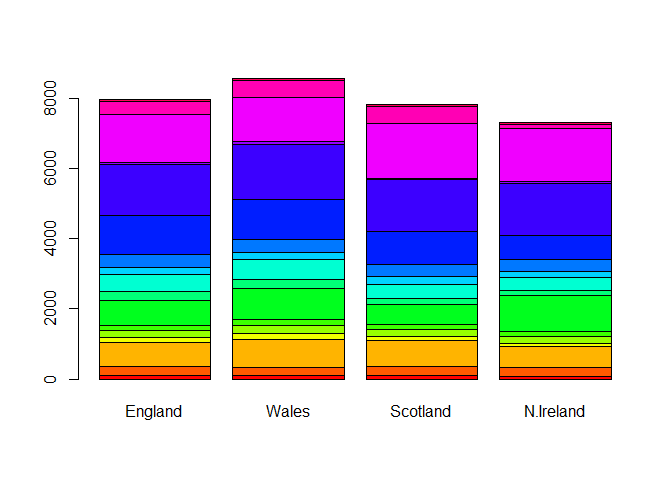
\includegraphics{class18_files/figure-pdf/unnamed-chunk-19-1.pdf}

}

\end{figure}

These groups are statistically different.

Get more data from CMI-PB

\begin{Shaded}
\begin{Highlighting}[]
\NormalTok{specimen }\OtherTok{\textless{}{-}} \FunctionTok{read\_json}\NormalTok{(}\StringTok{"https://www.cmi{-}pb.org/api/specimen"}\NormalTok{, }\AttributeTok{simplifyVector =}\NormalTok{ T)}
\FunctionTok{head}\NormalTok{(specimen)}
\end{Highlighting}
\end{Shaded}

\begin{verbatim}
  specimen_id subject_id actual_day_relative_to_boost
1           1          1                           -3
2           2          1                            1
3           3          1                            3
4           4          1                            7
5           5          1                           11
6           6          1                           32
  planned_day_relative_to_boost specimen_type visit
1                             0         Blood     1
2                             1         Blood     2
3                             3         Blood     3
4                             7         Blood     4
5                            14         Blood     5
6                            30         Blood     6
\end{verbatim}

We need to \textbf{join} these two tables (subject and specimen) to make
a single new ``meta'' table with all our metadata. We will use the
\texttt{dplyr} join functions to do this.

\begin{Shaded}
\begin{Highlighting}[]
\FunctionTok{library}\NormalTok{(dplyr)}
\end{Highlighting}
\end{Shaded}

\begin{quote}
Q9. Join specimen and subject tables to make a new merged data frame
containing all specimen records along with their associated subject
details:
\end{quote}

\begin{Shaded}
\begin{Highlighting}[]
\NormalTok{meta }\OtherTok{\textless{}{-}} \FunctionTok{inner\_join}\NormalTok{(subject, specimen)}
\end{Highlighting}
\end{Shaded}

\begin{verbatim}
Joining with `by = join_by(subject_id)`
\end{verbatim}

\begin{Shaded}
\begin{Highlighting}[]
\FunctionTok{head}\NormalTok{(meta)}
\end{Highlighting}
\end{Shaded}

\begin{verbatim}
  subject_id infancy_vac biological_sex              ethnicity  race
1          1          wP         Female Not Hispanic or Latino White
2          1          wP         Female Not Hispanic or Latino White
3          1          wP         Female Not Hispanic or Latino White
4          1          wP         Female Not Hispanic or Latino White
5          1          wP         Female Not Hispanic or Latino White
6          1          wP         Female Not Hispanic or Latino White
  year_of_birth date_of_boost      dataset      age specimen_id
1    1986-01-01    2016-09-12 2020_dataset 38.17933           1
2    1986-01-01    2016-09-12 2020_dataset 38.17933           2
3    1986-01-01    2016-09-12 2020_dataset 38.17933           3
4    1986-01-01    2016-09-12 2020_dataset 38.17933           4
5    1986-01-01    2016-09-12 2020_dataset 38.17933           5
6    1986-01-01    2016-09-12 2020_dataset 38.17933           6
  actual_day_relative_to_boost planned_day_relative_to_boost specimen_type
1                           -3                             0         Blood
2                            1                             1         Blood
3                            3                             3         Blood
4                            7                             7         Blood
5                           11                            14         Blood
6                           32                            30         Blood
  visit
1     1
2     2
3     3
4     4
5     5
6     6
\end{verbatim}

Now we can read some of the other data from CMI-PB.

\begin{Shaded}
\begin{Highlighting}[]
\NormalTok{ab\_titer }\OtherTok{\textless{}{-}} \FunctionTok{read\_json}\NormalTok{(}\StringTok{"https://www.cmi{-}pb.org/api/plasma\_ab\_titer"}\NormalTok{, }\AttributeTok{simplifyVector =}\NormalTok{ T)}
\FunctionTok{head}\NormalTok{(ab\_titer)}
\end{Highlighting}
\end{Shaded}

\begin{verbatim}
  specimen_id isotype is_antigen_specific antigen        MFI MFI_normalised
1           1     IgE               FALSE   Total 1110.21154       2.493425
2           1     IgE               FALSE   Total 2708.91616       2.493425
3           1     IgG                TRUE      PT   68.56614       3.736992
4           1     IgG                TRUE     PRN  332.12718       2.602350
5           1     IgG                TRUE     FHA 1887.12263      34.050956
6           1     IgE                TRUE     ACT    0.10000       1.000000
   unit lower_limit_of_detection
1 UG/ML                 2.096133
2 IU/ML                29.170000
3 IU/ML                 0.530000
4 IU/ML                 6.205949
5 IU/ML                 4.679535
6 IU/ML                 2.816431
\end{verbatim}

\begin{quote}
Q10. Now using the same procedure join meta with titer data so we can
further analyze this data in terms of time of visit aP/wP, male/female
etc.
\end{quote}

One more \texttt{inner\_join()} to add all our metadata in \texttt{meta}
on to our \texttt{ab\_data} table:

\begin{Shaded}
\begin{Highlighting}[]
\NormalTok{abdata }\OtherTok{\textless{}{-}} \FunctionTok{inner\_join}\NormalTok{(ab\_titer, meta)}
\end{Highlighting}
\end{Shaded}

\begin{verbatim}
Joining with `by = join_by(specimen_id)`
\end{verbatim}

\begin{Shaded}
\begin{Highlighting}[]
\FunctionTok{head}\NormalTok{(abdata)}
\end{Highlighting}
\end{Shaded}

\begin{verbatim}
  specimen_id isotype is_antigen_specific antigen        MFI MFI_normalised
1           1     IgE               FALSE   Total 1110.21154       2.493425
2           1     IgE               FALSE   Total 2708.91616       2.493425
3           1     IgG                TRUE      PT   68.56614       3.736992
4           1     IgG                TRUE     PRN  332.12718       2.602350
5           1     IgG                TRUE     FHA 1887.12263      34.050956
6           1     IgE                TRUE     ACT    0.10000       1.000000
   unit lower_limit_of_detection subject_id infancy_vac biological_sex
1 UG/ML                 2.096133          1          wP         Female
2 IU/ML                29.170000          1          wP         Female
3 IU/ML                 0.530000          1          wP         Female
4 IU/ML                 6.205949          1          wP         Female
5 IU/ML                 4.679535          1          wP         Female
6 IU/ML                 2.816431          1          wP         Female
               ethnicity  race year_of_birth date_of_boost      dataset
1 Not Hispanic or Latino White    1986-01-01    2016-09-12 2020_dataset
2 Not Hispanic or Latino White    1986-01-01    2016-09-12 2020_dataset
3 Not Hispanic or Latino White    1986-01-01    2016-09-12 2020_dataset
4 Not Hispanic or Latino White    1986-01-01    2016-09-12 2020_dataset
5 Not Hispanic or Latino White    1986-01-01    2016-09-12 2020_dataset
6 Not Hispanic or Latino White    1986-01-01    2016-09-12 2020_dataset
       age actual_day_relative_to_boost planned_day_relative_to_boost
1 38.17933                           -3                             0
2 38.17933                           -3                             0
3 38.17933                           -3                             0
4 38.17933                           -3                             0
5 38.17933                           -3                             0
6 38.17933                           -3                             0
  specimen_type visit
1         Blood     1
2         Blood     1
3         Blood     1
4         Blood     1
5         Blood     1
6         Blood     1
\end{verbatim}

\begin{quote}
Q11. How many specimens (i.e.~entries in abdata) do we have for each
isotype?
\end{quote}

\begin{Shaded}
\begin{Highlighting}[]
\FunctionTok{table}\NormalTok{(abdata}\SpecialCharTok{$}\NormalTok{isotype)}
\end{Highlighting}
\end{Shaded}

\begin{verbatim}

 IgE  IgG IgG1 IgG2 IgG3 IgG4 
6698 4255 8983 8990 8990 8990 
\end{verbatim}

\begin{quote}
Q12. What are the different \$dataset values in abdata and what do you
notice about the number of rows for the most ``recent'' dataset?
\end{quote}

\begin{Shaded}
\begin{Highlighting}[]
\FunctionTok{table}\NormalTok{(abdata}\SpecialCharTok{$}\NormalTok{dataset)}
\end{Highlighting}
\end{Shaded}

\begin{verbatim}

2020_dataset 2021_dataset 2022_dataset 
       31520         8085         7301 
\end{verbatim}

There is a signficantly smaller amount of data for the more recent
datasets.

Our first exploratory plot:

\begin{Shaded}
\begin{Highlighting}[]
\FunctionTok{table}\NormalTok{(abdata}\SpecialCharTok{$}\NormalTok{antigen)}
\end{Highlighting}
\end{Shaded}

\begin{verbatim}

    ACT   BETV1      DT   FELD1     FHA  Fim2/3  FIM2/3   LOLP1     LOS Measles 
   1970    1970    4168    1970    4562    1043    3125    1970    1970    1970 
    OVA     PD1     PRN      PT     PTM   Total      TT 
   4168    1970    4562    4562    1970     788    4168 
\end{verbatim}

\begin{quote}
Q13. Make a summary boxplot of Ab titer levels (MFI) for all antigens:
\end{quote}

\begin{Shaded}
\begin{Highlighting}[]
\FunctionTok{ggplot}\NormalTok{(abdata) }\SpecialCharTok{+}
  \FunctionTok{aes}\NormalTok{(MFI, antigen) }\SpecialCharTok{+}
  \FunctionTok{geom\_boxplot}\NormalTok{()}
\end{Highlighting}
\end{Shaded}

\begin{verbatim}
Warning: Removed 1 rows containing non-finite values (`stat_boxplot()`).
\end{verbatim}

\begin{figure}[H]

{\centering 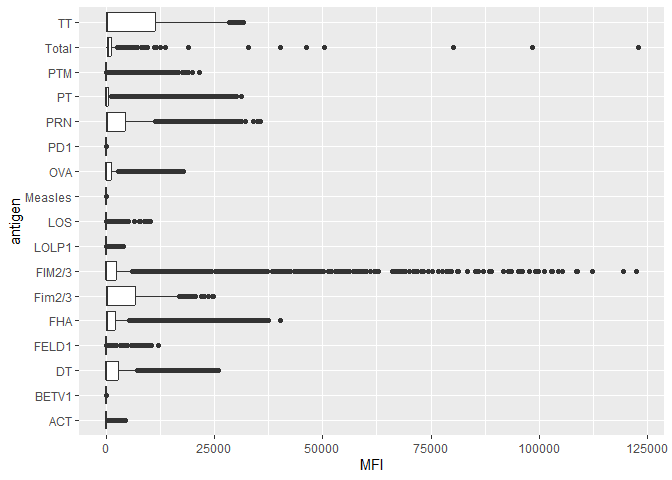
\includegraphics{class18_files/figure-pdf/unnamed-chunk-28-1.pdf}

}

\end{figure}

Can you facet or even just color by infancy\_vac? Is there some
difference?

\begin{Shaded}
\begin{Highlighting}[]
\FunctionTok{ggplot}\NormalTok{(abdata) }\SpecialCharTok{+}
  \FunctionTok{aes}\NormalTok{(MFI, antigen, }\AttributeTok{col =}\NormalTok{ infancy\_vac) }\SpecialCharTok{+}
  \FunctionTok{geom\_boxplot}\NormalTok{() }
\end{Highlighting}
\end{Shaded}

\begin{verbatim}
Warning: Removed 1 rows containing non-finite values (`stat_boxplot()`).
\end{verbatim}

\begin{figure}[H]

{\centering 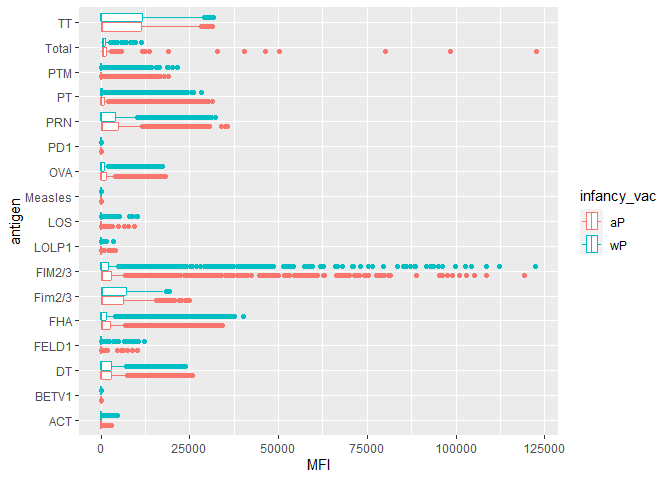
\includegraphics{class18_files/figure-pdf/unnamed-chunk-29-1.pdf}

}

\end{figure}

\begin{quote}
Q14. What antigens show differences in the level of IgG antibody titers
recognizing them over time? Why these and not others? Why are certain
antigens and not others very variable in their detected levels here?
\end{quote}

Different antigens have different proportions of the components within
the vaccine.

\begin{quote}
Q15. Filter to pull out only two specific antigens for analysis and
create a boxplot for each. You can chose any you like. Below I picked a
``control'' antigen (``OVA'', that is not in our vaccines) and a clear
antigen of interest (``PT'', Pertussis Toxin, one of the key virulence
factors produced by the bacterium B. pertussis) and the same for
antigen==``FIM2/3''.
\end{quote}

\begin{Shaded}
\begin{Highlighting}[]
\FunctionTok{filter}\NormalTok{(abdata, antigen}\SpecialCharTok{==}\StringTok{"OVA"}\NormalTok{) }\SpecialCharTok{\%\textgreater{}\%}
  \FunctionTok{ggplot}\NormalTok{() }\SpecialCharTok{+}
  \FunctionTok{aes}\NormalTok{(MFI\_normalised, }\AttributeTok{col=}\NormalTok{infancy\_vac) }\SpecialCharTok{+}
  \FunctionTok{geom\_boxplot}\NormalTok{(}\AttributeTok{show.legend =}\NormalTok{ T) }\SpecialCharTok{+}
  \FunctionTok{facet\_wrap}\NormalTok{(}\FunctionTok{vars}\NormalTok{(visit)) }\SpecialCharTok{+}
  \FunctionTok{theme\_bw}\NormalTok{()}
\end{Highlighting}
\end{Shaded}

\begin{figure}[H]

{\centering 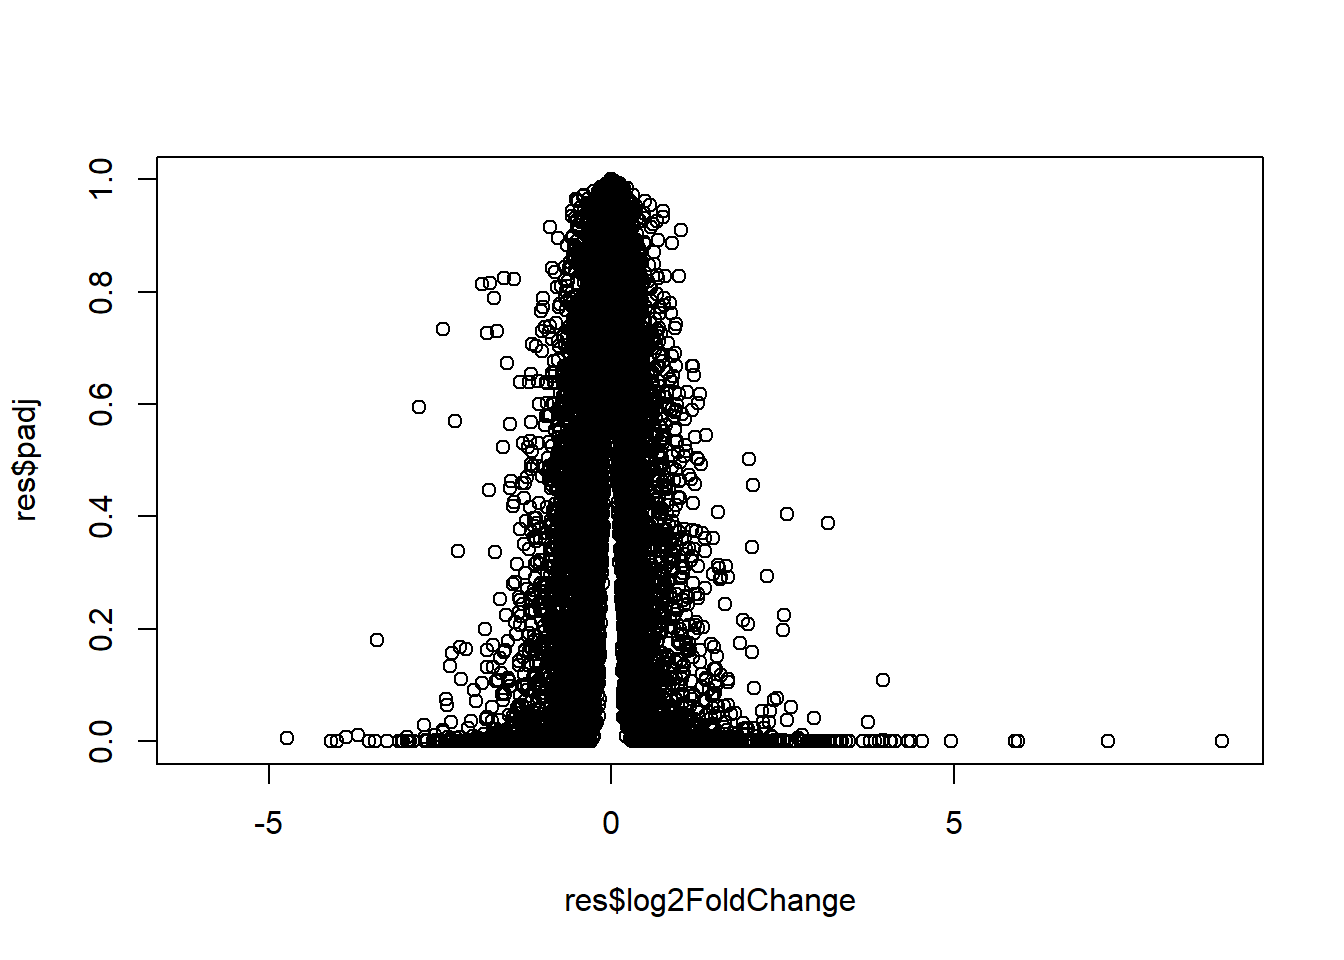
\includegraphics{class18_files/figure-pdf/unnamed-chunk-30-1.pdf}

}

\end{figure}

\begin{Shaded}
\begin{Highlighting}[]
\FunctionTok{filter}\NormalTok{(abdata, antigen}\SpecialCharTok{==}\StringTok{"FIM2/3"}\NormalTok{) }\SpecialCharTok{\%\textgreater{}\%}
  \FunctionTok{ggplot}\NormalTok{() }\SpecialCharTok{+}
  \FunctionTok{aes}\NormalTok{(MFI\_normalised, }\AttributeTok{col=}\NormalTok{infancy\_vac) }\SpecialCharTok{+}
  \FunctionTok{geom\_boxplot}\NormalTok{(}\AttributeTok{show.legend =}\NormalTok{ T ) }\SpecialCharTok{+}
  \FunctionTok{facet\_wrap}\NormalTok{(}\FunctionTok{vars}\NormalTok{(visit)) }\SpecialCharTok{+}
  \FunctionTok{theme\_bw}\NormalTok{()}
\end{Highlighting}
\end{Shaded}

\begin{figure}[H]

{\centering 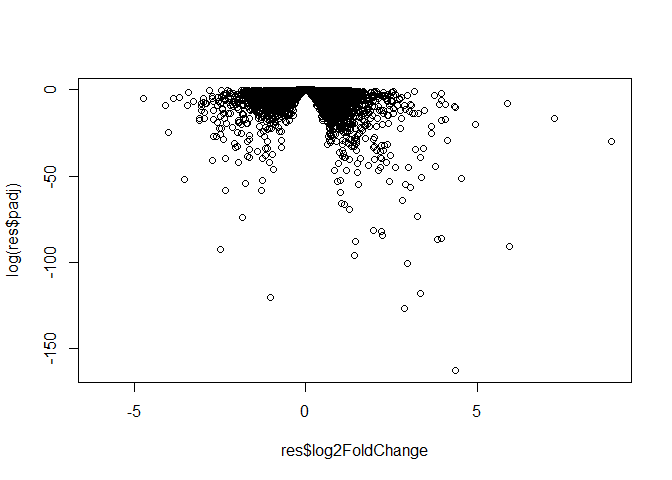
\includegraphics{class18_files/figure-pdf/unnamed-chunk-31-1.pdf}

}

\end{figure}

\begin{quote}
Q16: What do you notice about these two antigens time courses and the PT
data in particular?
\end{quote}

The PT levels rise over time at a higher level compared to OVA. There is
a similar trend for where wP and aP subjects peak.

There are potentially some differences here, but in general it is hard
to tell with this whole dataset overview\ldots{}

\begin{Shaded}
\begin{Highlighting}[]
\FunctionTok{table}\NormalTok{(abdata}\SpecialCharTok{$}\NormalTok{dataset)}
\end{Highlighting}
\end{Shaded}

\begin{verbatim}

2020_dataset 2021_dataset 2022_dataset 
       31520         8085         7301 
\end{verbatim}

Let's focus in on just the 2021\_dataset.

\begin{Shaded}
\begin{Highlighting}[]
\NormalTok{abdata}\FloatTok{.21} \OtherTok{\textless{}{-}} \FunctionTok{filter}\NormalTok{(abdata, dataset }\SpecialCharTok{==} \StringTok{"2021\_dataset"}\NormalTok{)}
\FunctionTok{table}\NormalTok{(abdata}\FloatTok{.21}\SpecialCharTok{$}\NormalTok{dataset)}
\end{Highlighting}
\end{Shaded}

\begin{verbatim}

2021_dataset 
        8085 
\end{verbatim}

Focus on PT antigen for IgG levels.

\begin{Shaded}
\begin{Highlighting}[]
\NormalTok{pt}\FloatTok{.21} \OtherTok{\textless{}{-}} \FunctionTok{filter}\NormalTok{(abdata}\FloatTok{.21}\NormalTok{, isotype }\SpecialCharTok{==} \StringTok{"IgG"}\NormalTok{, antigen }\SpecialCharTok{==} \StringTok{"PT"}\NormalTok{)}
\end{Highlighting}
\end{Shaded}

Plot of days (time) relative to boost vs MFI levels.

\begin{Shaded}
\begin{Highlighting}[]
\FunctionTok{ggplot}\NormalTok{(pt}\FloatTok{.21}\NormalTok{) }\SpecialCharTok{+}
  \FunctionTok{aes}\NormalTok{(}\AttributeTok{x=}\NormalTok{planned\_day\_relative\_to\_boost,}
        \AttributeTok{y=}\NormalTok{MFI\_normalised,}
        \AttributeTok{col=}\NormalTok{infancy\_vac) }\SpecialCharTok{+}
  \FunctionTok{geom\_point}\NormalTok{()}
\end{Highlighting}
\end{Shaded}

\begin{figure}[H]

{\centering 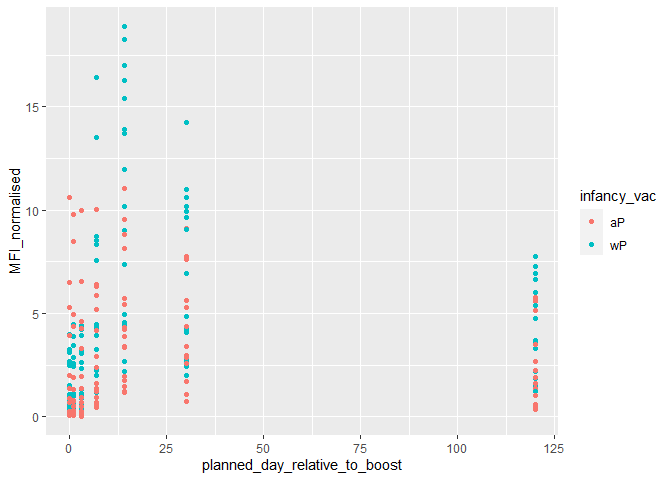
\includegraphics{class18_files/figure-pdf/unnamed-chunk-35-1.pdf}

}

\end{figure}

\begin{Shaded}
\begin{Highlighting}[]
\FunctionTok{ggplot}\NormalTok{(pt}\FloatTok{.21}\NormalTok{) }\SpecialCharTok{+}
  \FunctionTok{aes}\NormalTok{(}\AttributeTok{x=}\NormalTok{planned\_day\_relative\_to\_boost,}
        \AttributeTok{y=}\NormalTok{MFI\_normalised,}
        \AttributeTok{col=}\NormalTok{infancy\_vac,}
        \AttributeTok{group=}\NormalTok{subject\_id) }\SpecialCharTok{+}
  \FunctionTok{geom\_point}\NormalTok{() }\SpecialCharTok{+}
  \FunctionTok{geom\_line}\NormalTok{()}
\end{Highlighting}
\end{Shaded}

\begin{figure}[H]

{\centering 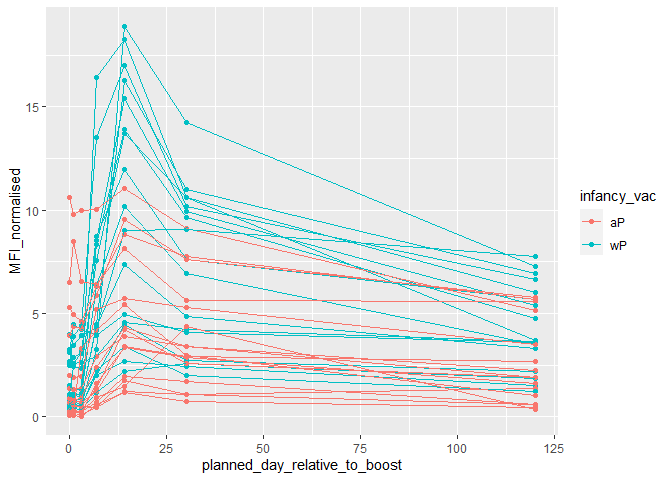
\includegraphics{class18_files/figure-pdf/unnamed-chunk-36-1.pdf}

}

\end{figure}

\begin{Shaded}
\begin{Highlighting}[]
\FunctionTok{ggplot}\NormalTok{(pt}\FloatTok{.21}\NormalTok{) }\SpecialCharTok{+}
  \FunctionTok{aes}\NormalTok{(}\AttributeTok{x=}\NormalTok{planned\_day\_relative\_to\_boost,}
        \AttributeTok{y=}\NormalTok{MFI\_normalised,}
        \AttributeTok{col=}\NormalTok{infancy\_vac,}
        \AttributeTok{group=}\NormalTok{subject\_id) }\SpecialCharTok{+}
  \FunctionTok{geom\_point}\NormalTok{() }\SpecialCharTok{+}
  \FunctionTok{geom\_line}\NormalTok{() }\SpecialCharTok{+}
  \FunctionTok{geom\_vline}\NormalTok{(}\AttributeTok{xintercept=}\DecValTok{0}\NormalTok{, }\AttributeTok{linetype=}\StringTok{"dashed"}\NormalTok{) }\SpecialCharTok{+}
  \FunctionTok{geom\_vline}\NormalTok{(}\AttributeTok{xintercept=}\DecValTok{14}\NormalTok{, }\AttributeTok{linetype=}\StringTok{"dashed"}\NormalTok{) }\SpecialCharTok{+}
  \FunctionTok{labs}\NormalTok{(}\AttributeTok{title=}\StringTok{"2021 dataset IgG PT"}\NormalTok{,}
       \AttributeTok{subtitle =} \StringTok{"Dashed lines indicate day 0 (pre{-}boost) and 14 (apparent peak levels)"}\NormalTok{)}
\end{Highlighting}
\end{Shaded}

\begin{figure}[H]

{\centering 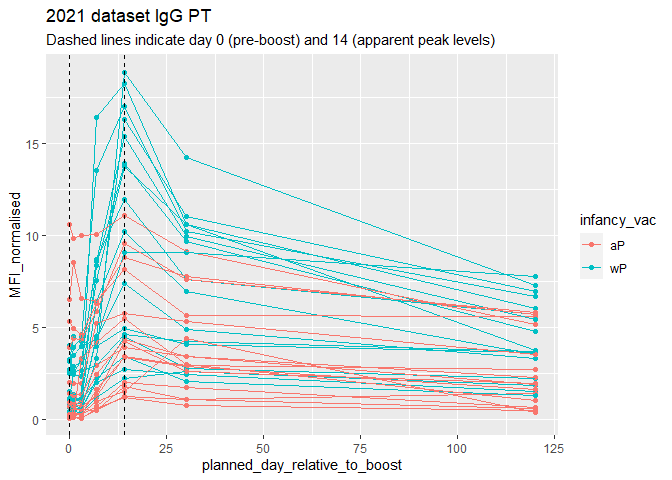
\includegraphics{class18_files/figure-pdf/unnamed-chunk-37-1.pdf}

}

\end{figure}

\begin{quote}
Q17: Do you see any clear difference in aP vs.~wP responses?
\end{quote}

The levels of MFI reach significantly higher peaks in wP individuals
compared to aP individuals at day 14. The levels are less distinct as
more time passes, with wP still showing higher MFI levels on average.



\end{document}
